% Appendix X

\chapter{Raw multiplicity analysis}\label{app:mult}

%----------------------------------------------------------------------------------------

\section{Effect of the rescue procedure on the multiplicity sum}

An other way to look at the effect of the rescue procedure is through the multiplicity sum. Dividing the multiplicities in four bins of target, the multiplicity sum should be the same in all bins of target. Before the rescue procedure one can see that this is not the case as the multiplicity sum for the last part of the target is consistently smaller as seen in Fig.~\ref{pic:ZApp}. After the rescue procedure however, the result is as expected.

\begin{figure}[!h]
  \centering
	\subfloat[]{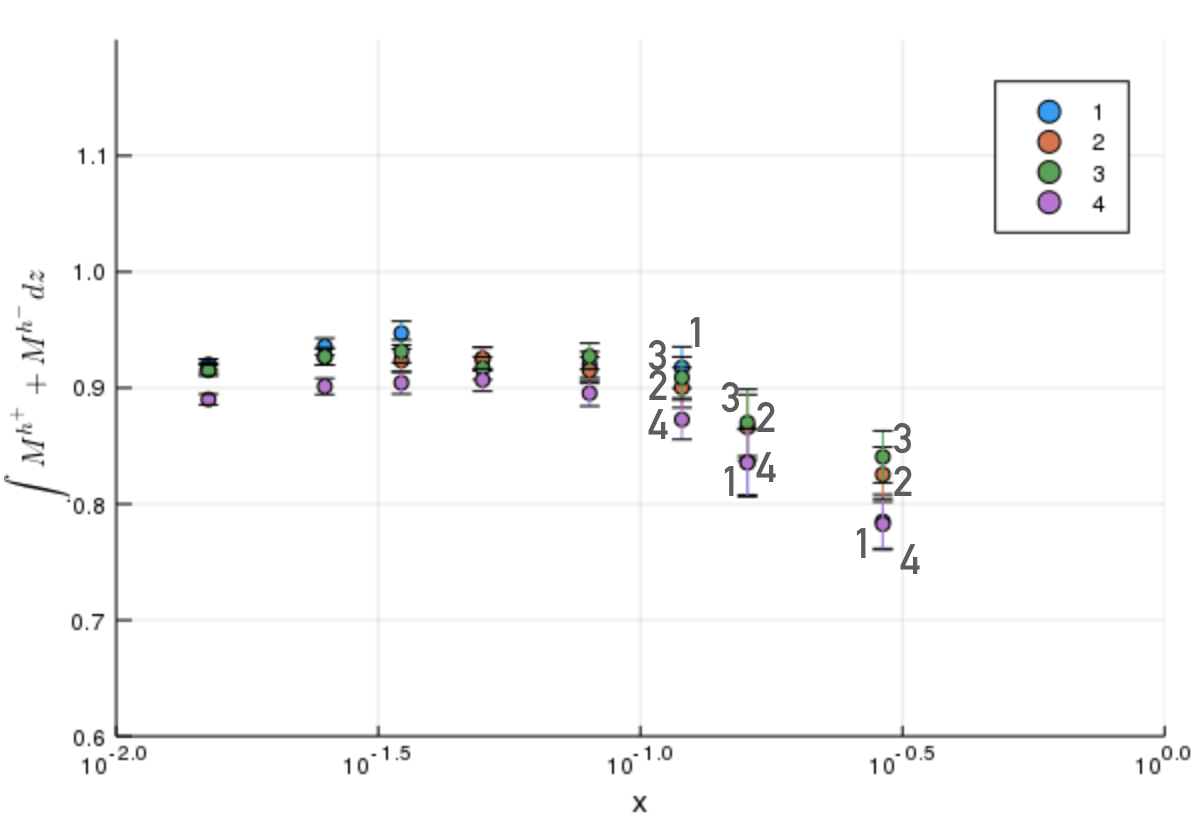
\includegraphics[scale=0.5]{./gfx/SumVertexB4RP.png}} \\
  \subfloat[]{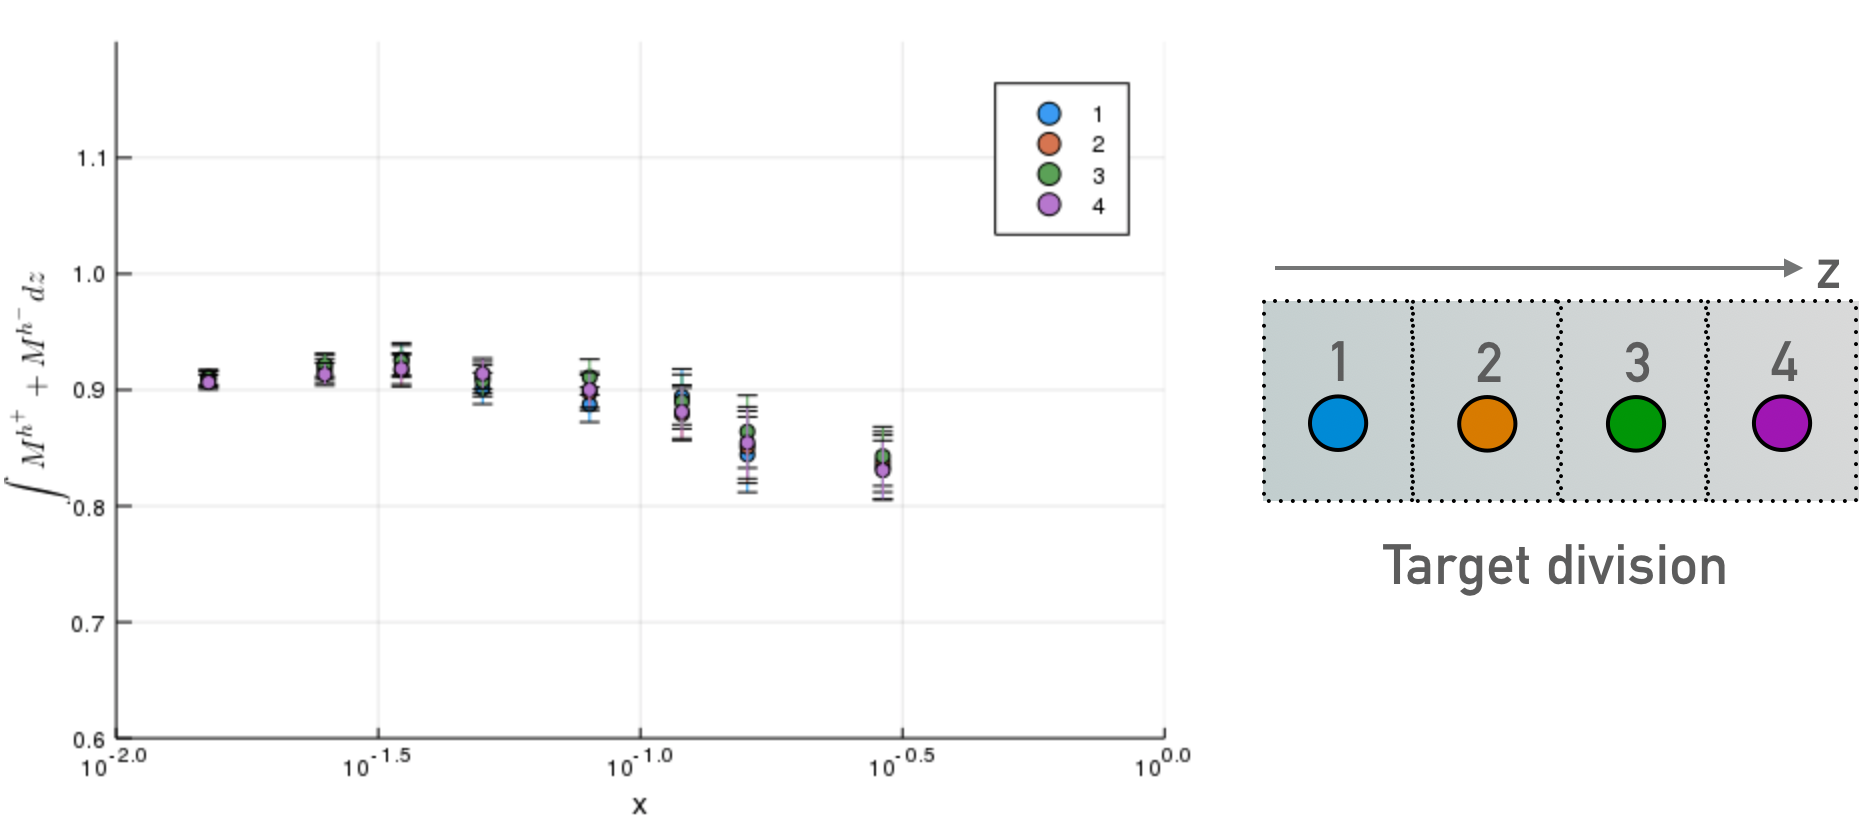
\includegraphics[scale=0.5]{./gfx/SumVertexBis.png}}
	\caption{Comparison of the multiplicity sum before the application of the rescue procedure (a) and after (b) for different target slices.}
	\label{pic:ZApp}
\end{figure}

%----------------------------------------------------------------------------------------

\section{Results for raw multiplicities of identified hadrons}

The raw multiplicity results shown in this section are without any correction except the RICH unfolding correction for identified hadrons. The unidentified hadron multiplicities are displayed as a function of $z$ in bins of $x$ and staggered vertically with $y$ in Figs.~\ref{pic:rawpip} to \ref{pic:rawpm}. The charged hadron multiplicities strongly depends on $z$ as expected with a small dependence with $x$ also.

\newpage

\begin{figure}[!h]
  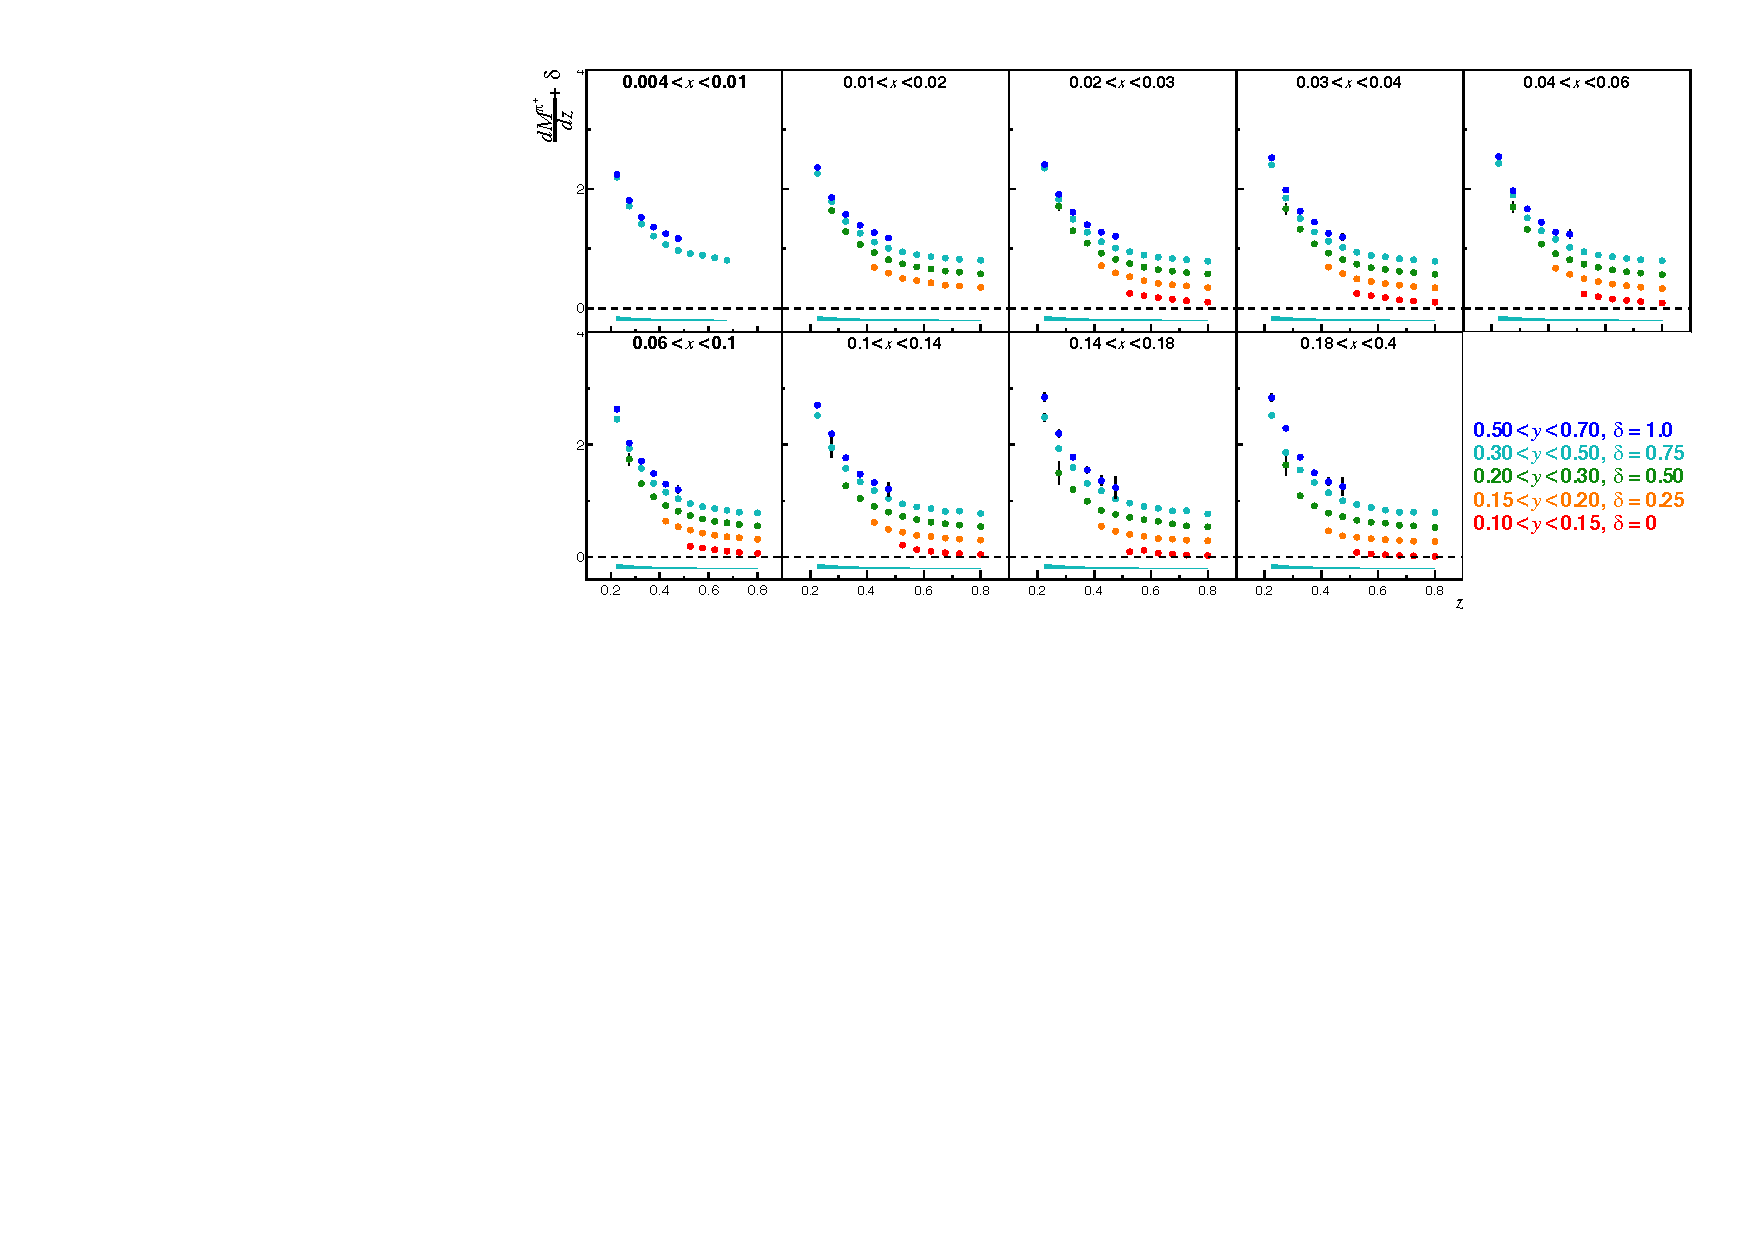
\includegraphics[scale=0.85]{./gfx/rawpip.pdf}
  \caption{Same as Fig.~\ref{pic:rawhp} but for positive pions.}
  \label{pic:rawpip}
\end{figure}

\begin{figure}[!h]
  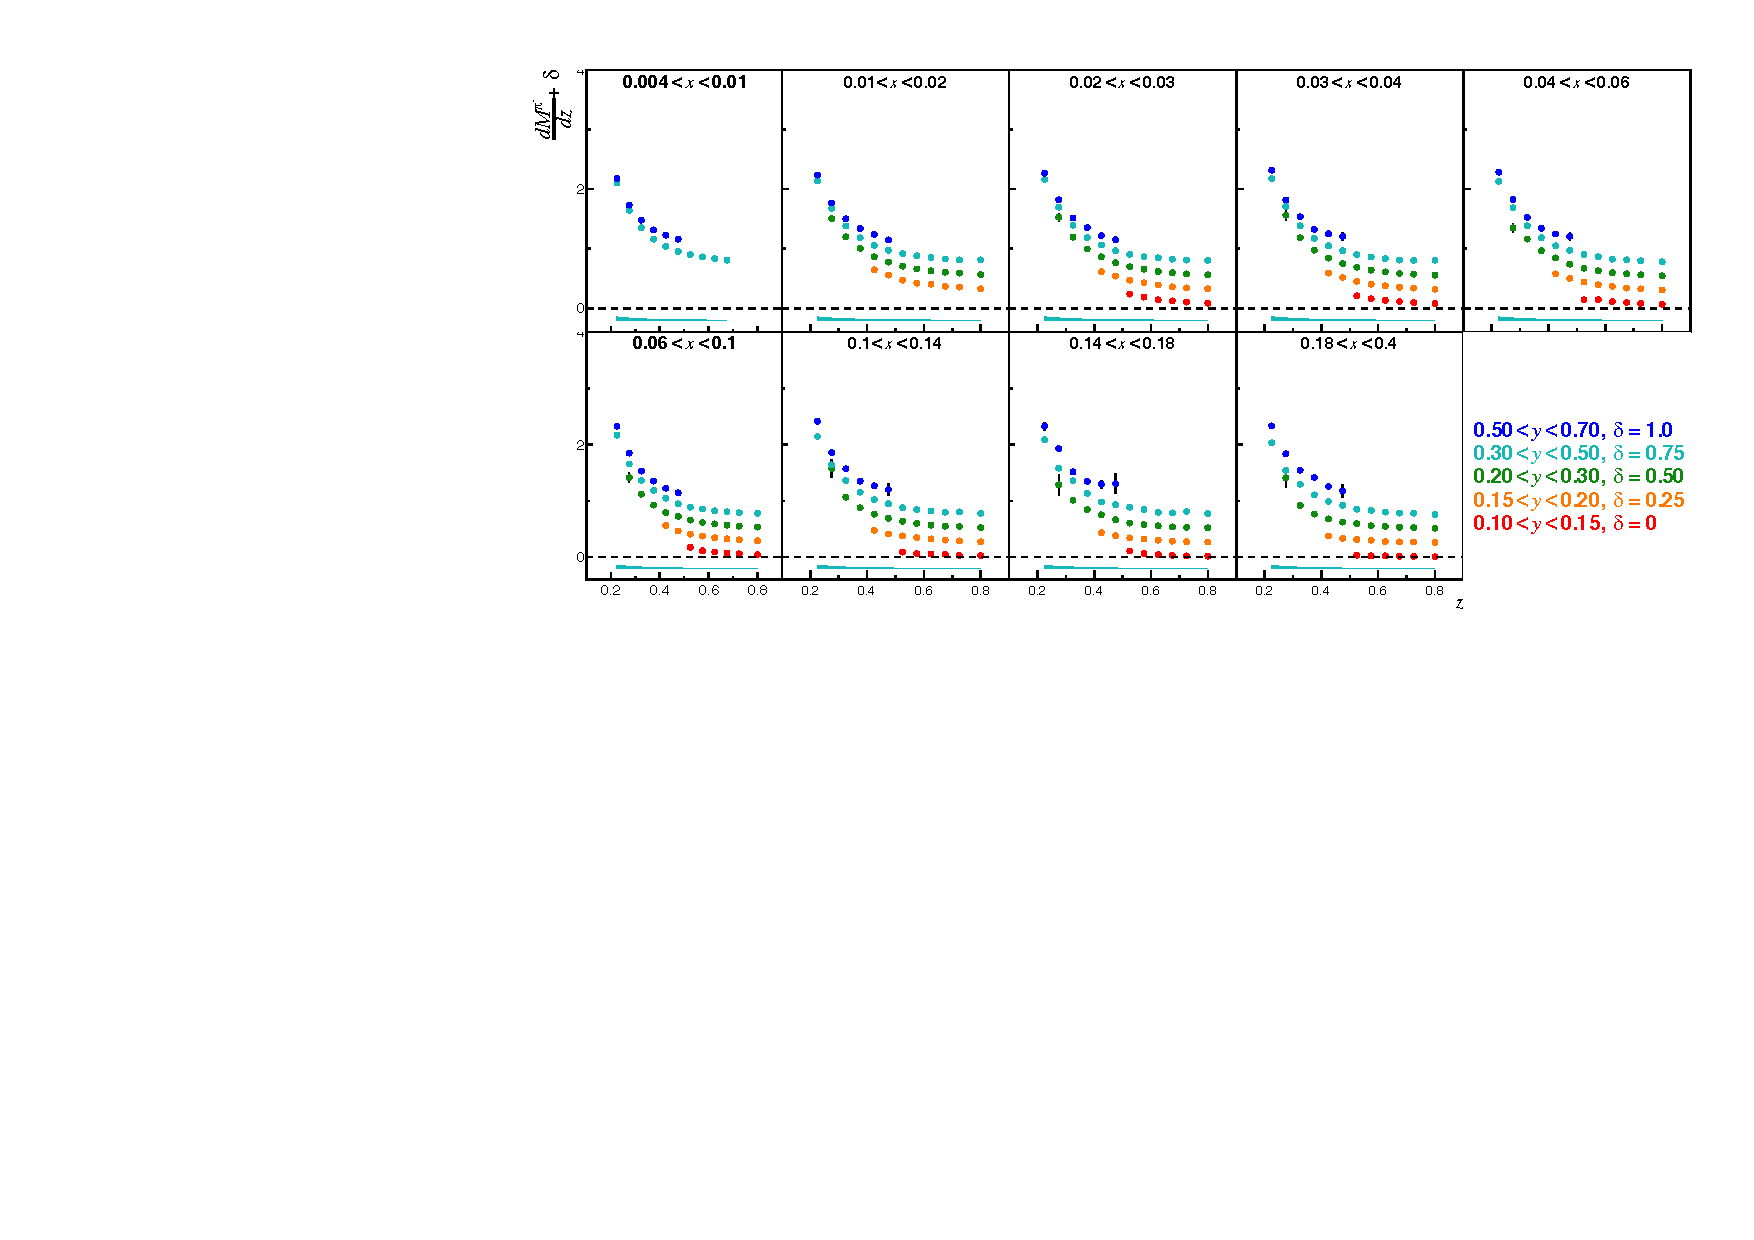
\includegraphics[scale=0.85]{./gfx/rawpim.pdf}
  \caption{Same as Fig.~\ref{pic:rawhp} but for negative pions.}
  \label{pic:rawpim}
\end{figure}

\newpage

\begin{figure}[!h]
  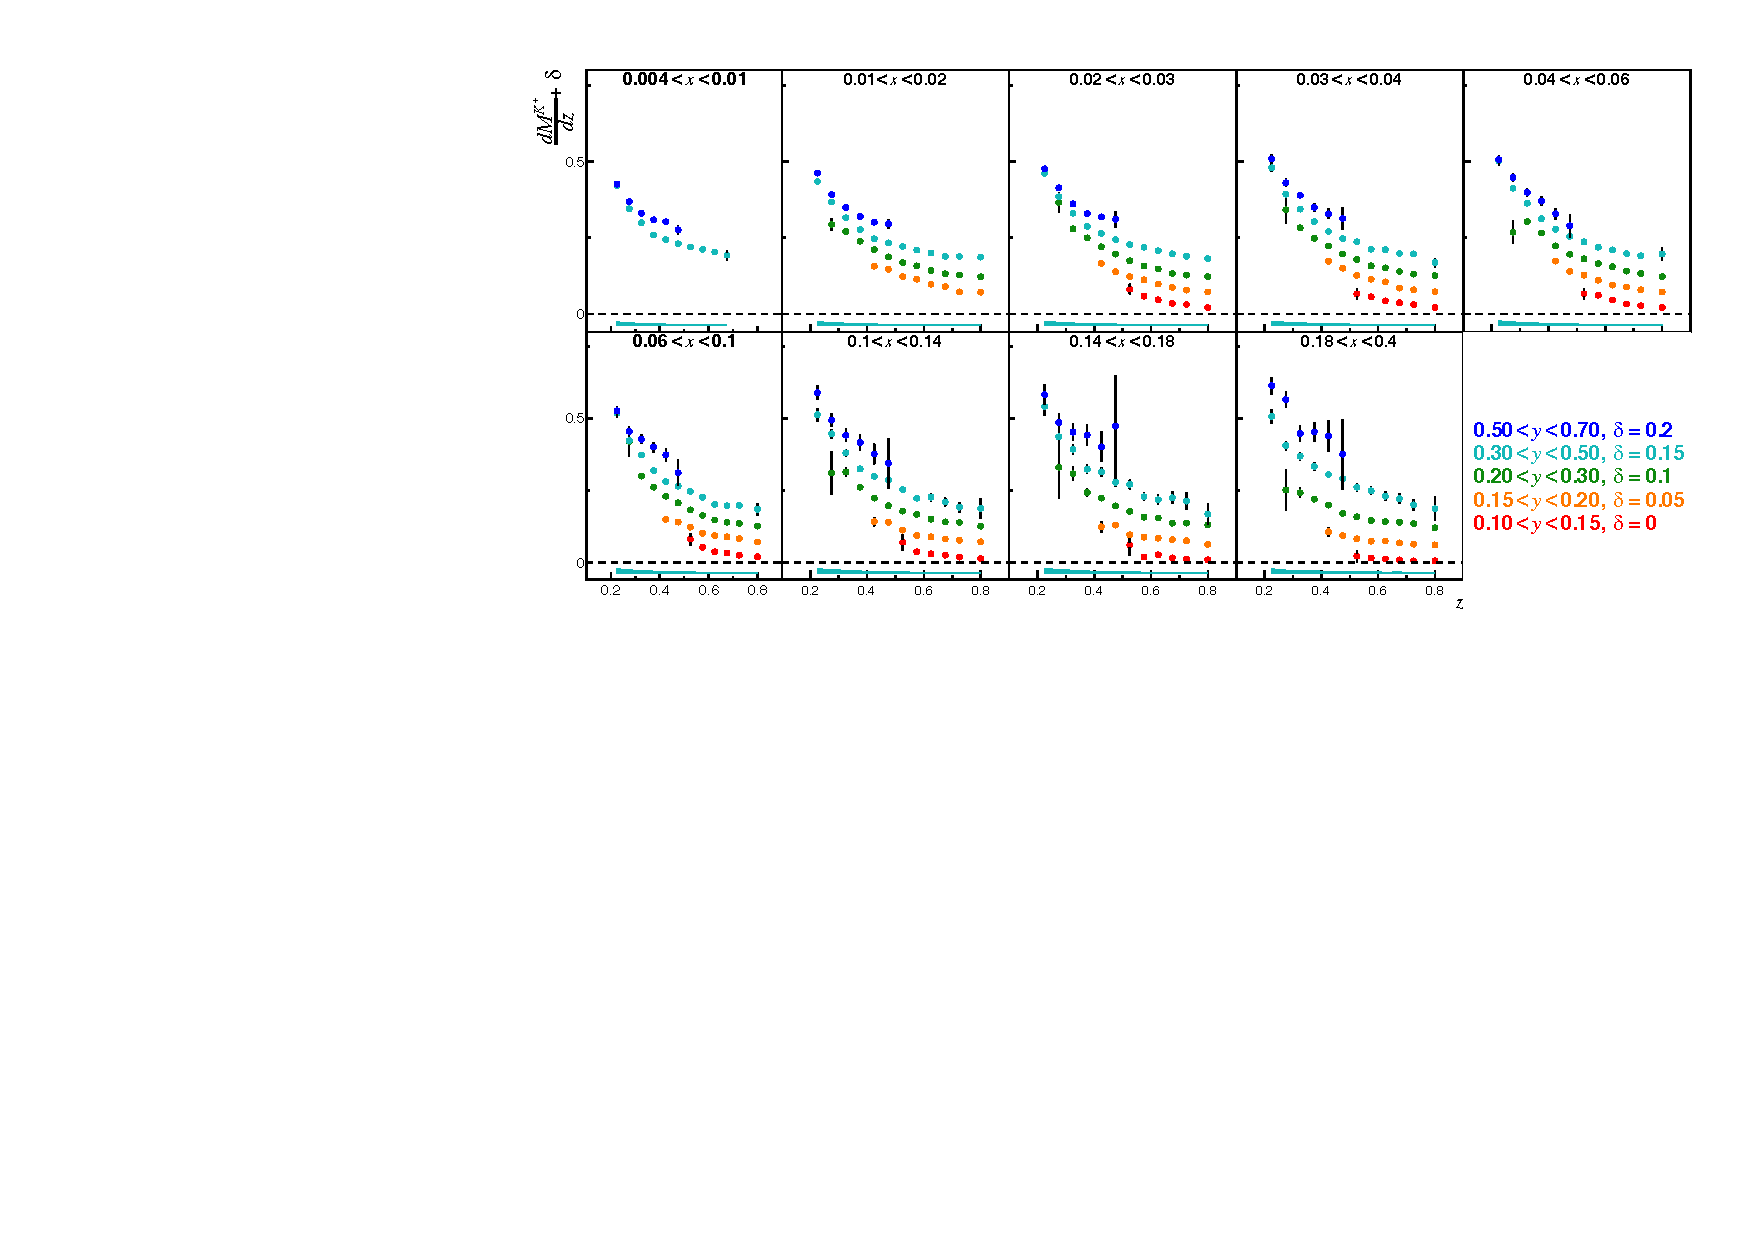
\includegraphics[scale=0.85]{./gfx/rawkp.pdf}
  \caption{Same as Fig.~\ref{pic:rawhp} but for positive kaons.}
  \label{pic:rawkp}
\end{figure}

\begin{figure}[!h]
  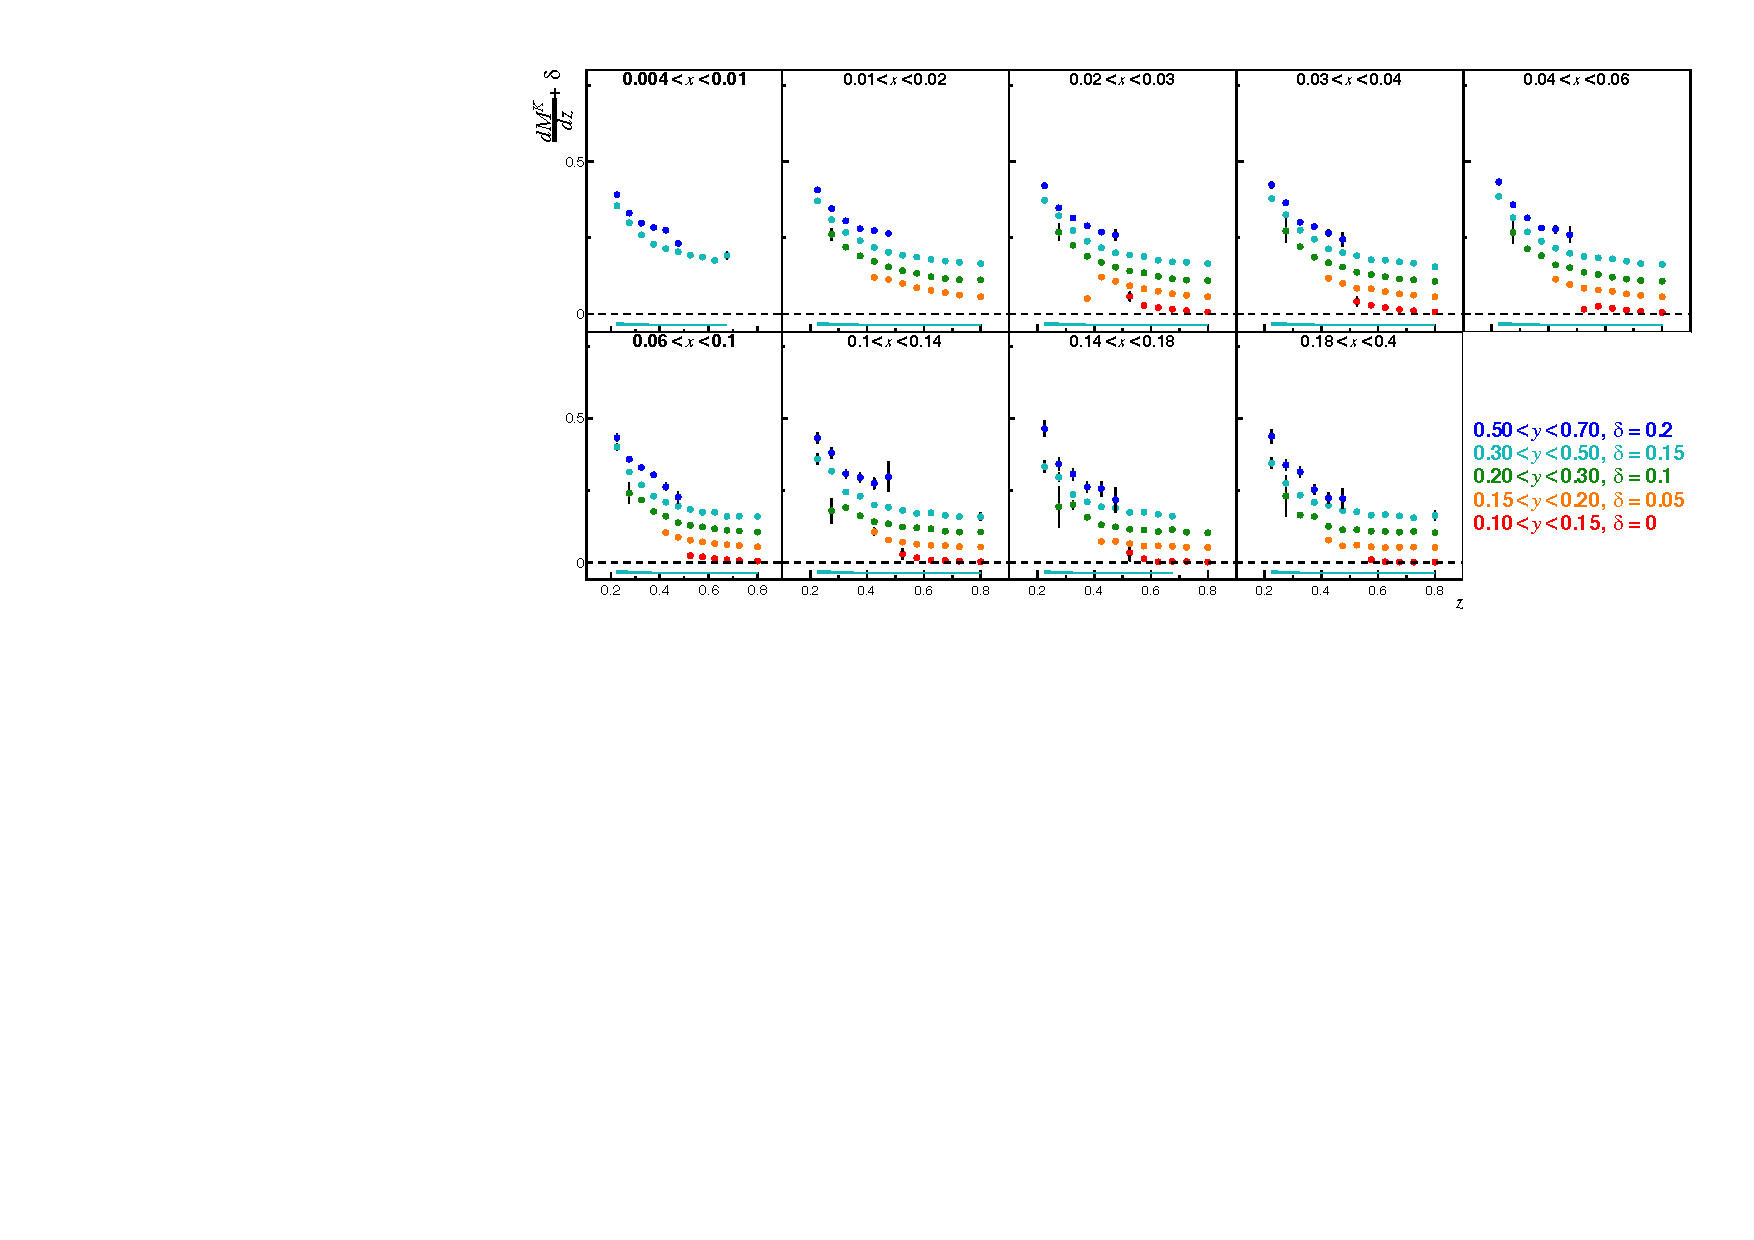
\includegraphics[scale=0.85]{./gfx/rawkm.pdf}
  \caption{Same as Fig.~\ref{pic:rawhp} but for negative pions.}
  \label{pic:rawkm}
\end{figure}

\newpage

\begin{figure}[!h]
  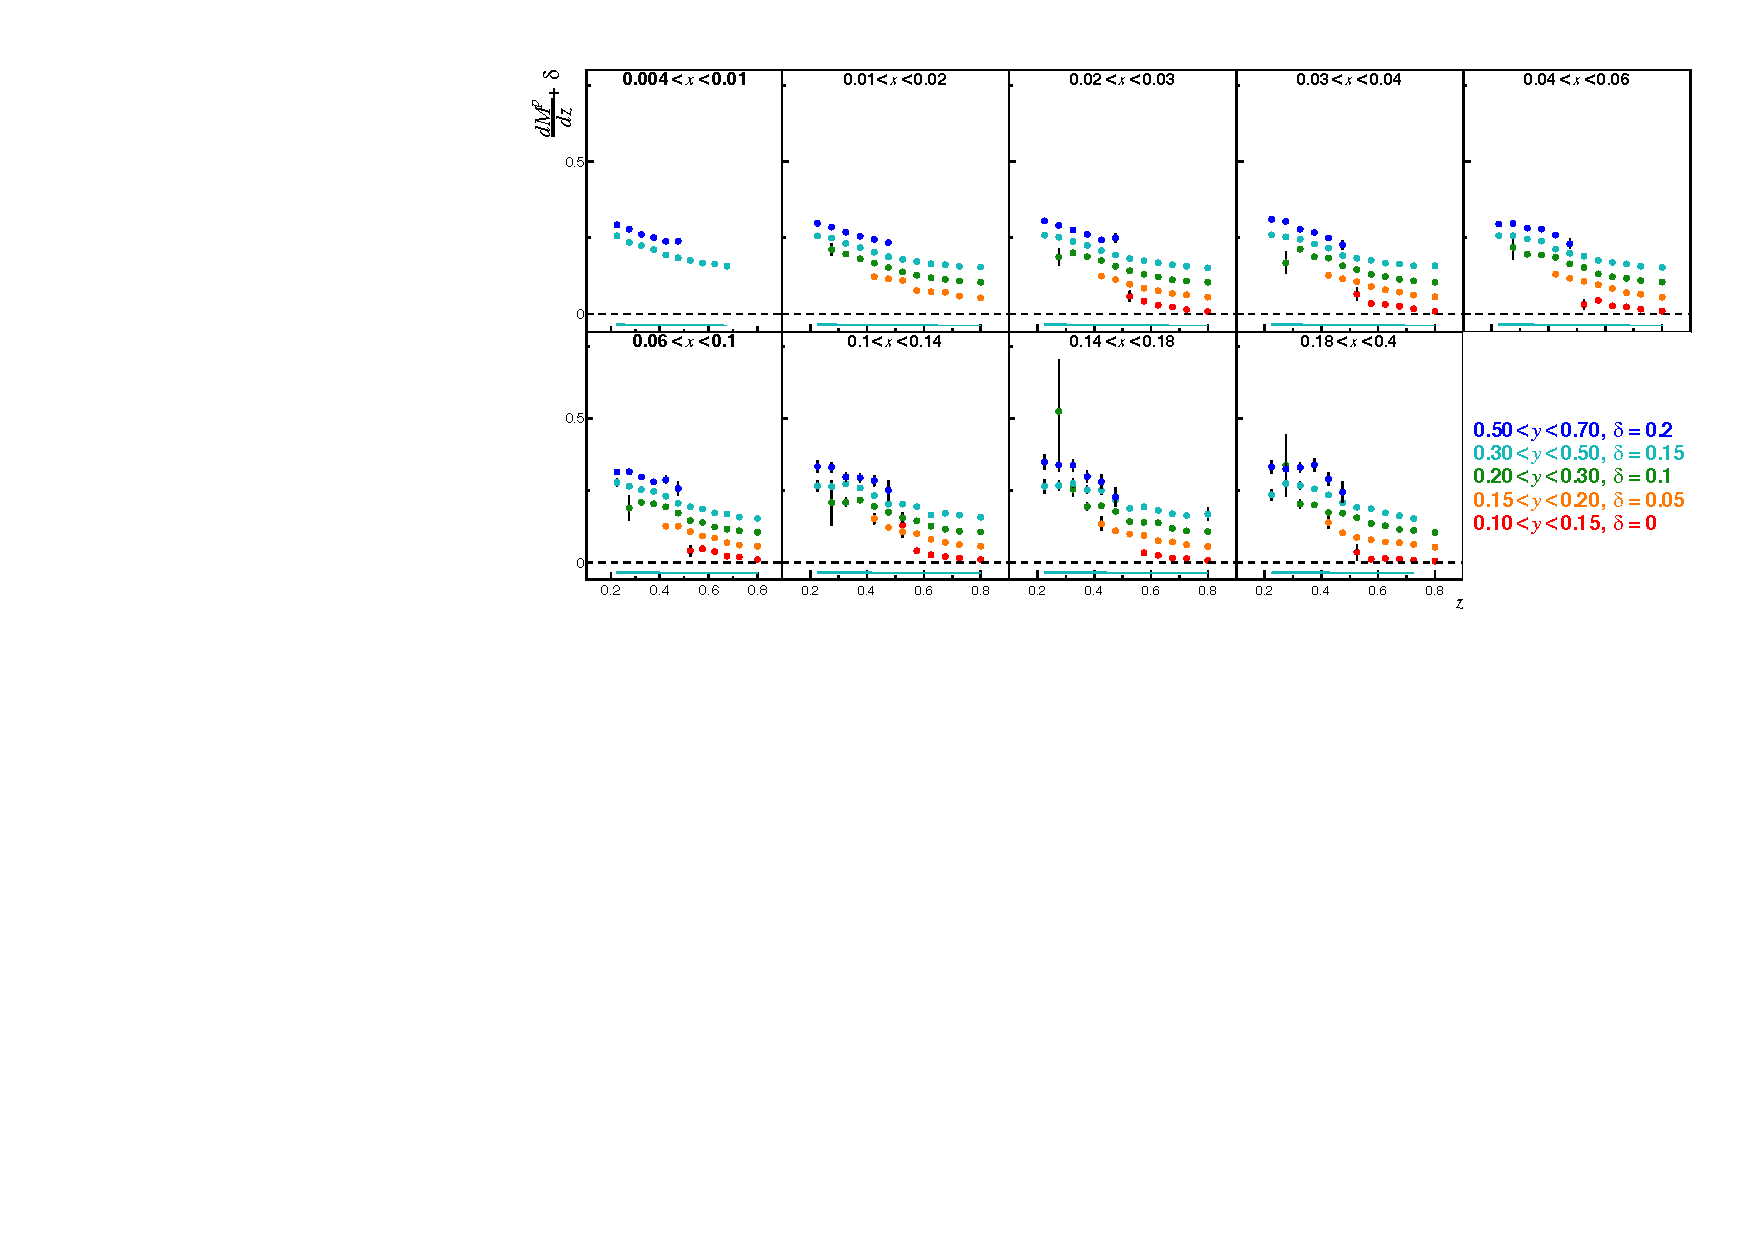
\includegraphics[scale=0.85]{./gfx/rawpp.pdf}
  \caption{Same as Fig.~\ref{pic:rawhp} but for protons.}
  \label{pic:rawpp}
\end{figure}

\begin{figure}[!h]
  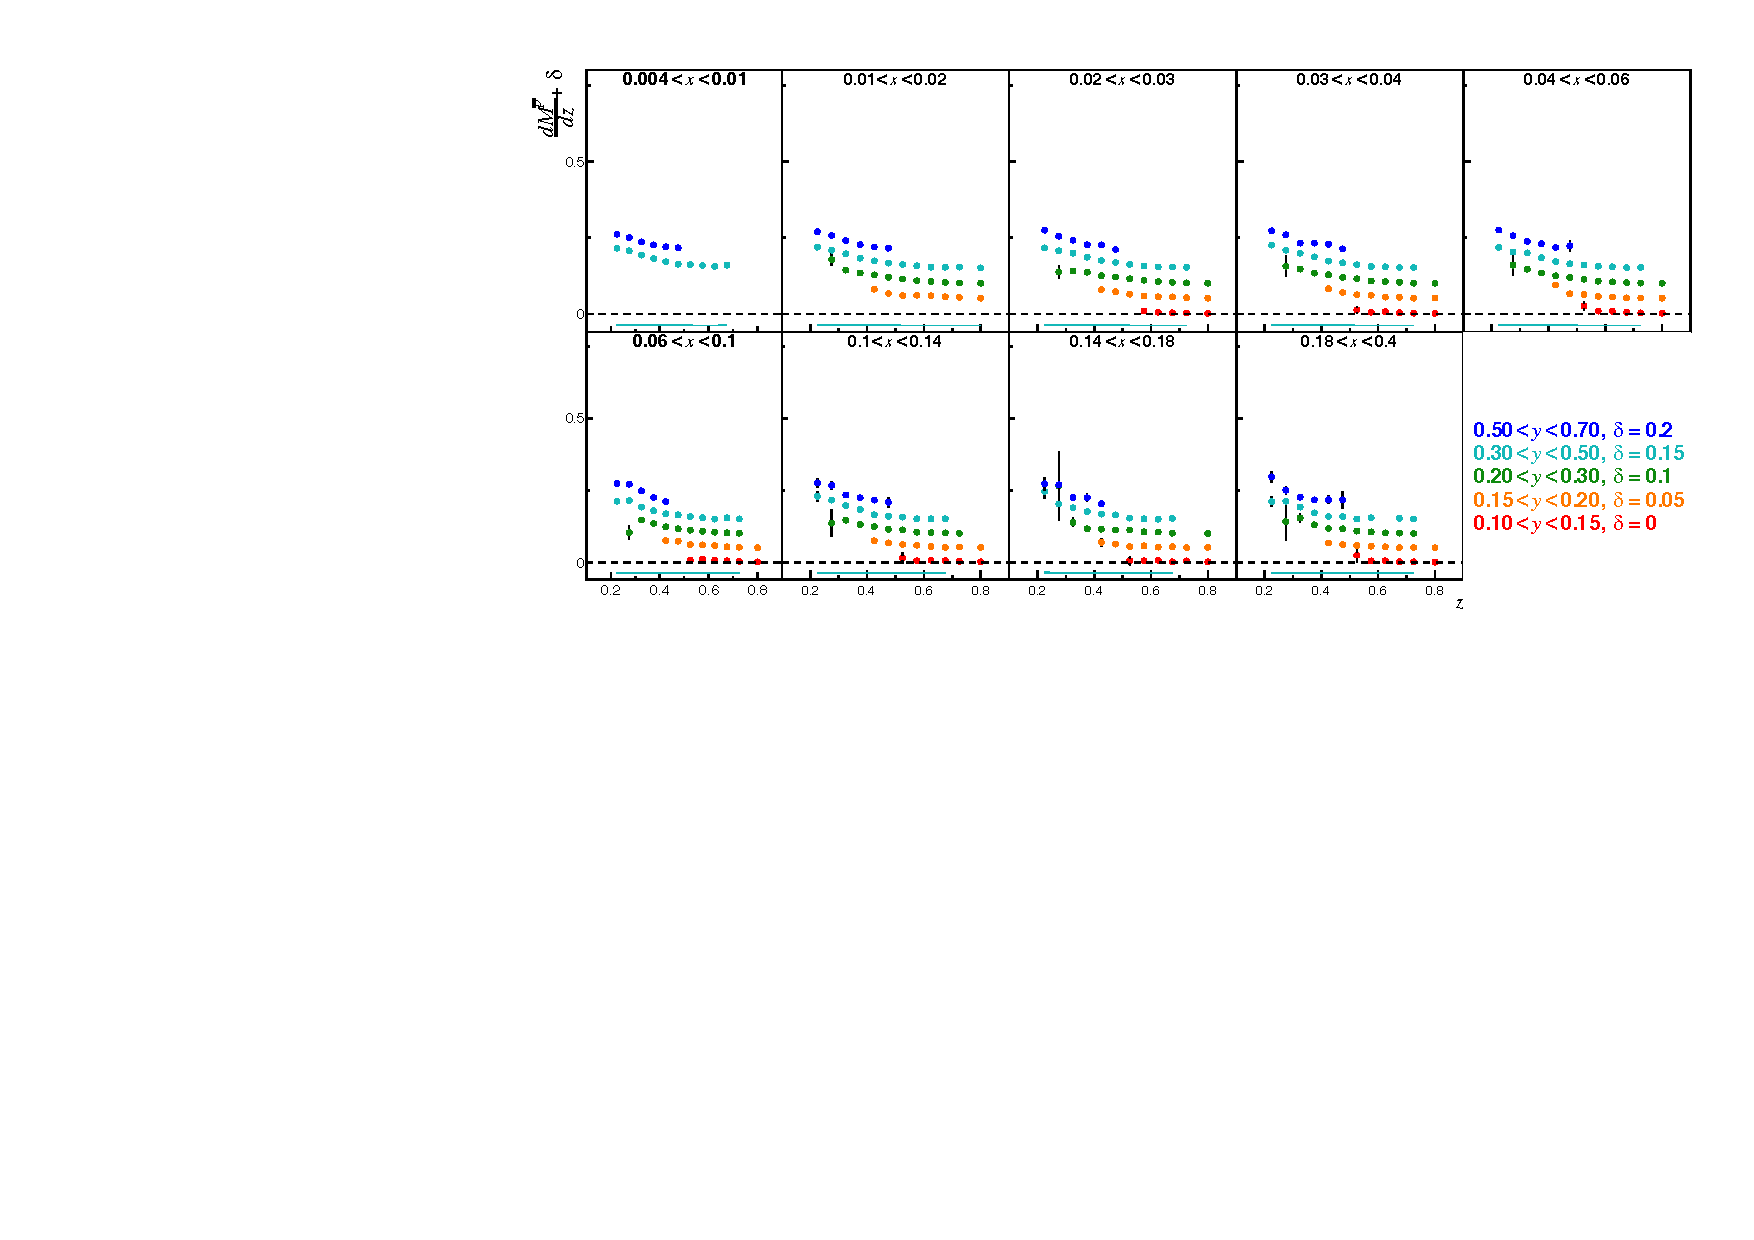
\includegraphics[scale=0.85]{./gfx/rawpm.pdf}
  \caption{Same as Fig.~\ref{pic:rawhp} but for antiprotons.}
  \label{pic:rawpm}
\end{figure}
